%\documentclass[12pt,twoside]{article}
\documentclass[conference]{IEEEtran}  % this should work with your LaTeX installation; else download extra package (www.ctan.org/pkg/ieeetran) or remove IEEE usage below

%%%%%%% Fill this out:
\newcommand{\trtitle}{Detecting Opinion Spammer Groups}
\newcommand{\titleshort}{NNs for Artificial Agents} % title for header:
\newcommand{\authorlastnames}{Adams, Jefferson, Washington} % alphabetical for seminars
\newcommand{\trcourse}{Knowledge Processing in Intelligent Systems: Practical Seminar}
\newcommand{\trgroup}{Knowledge Technology, WTM}
\newcommand{\truniversity}{Department of Informatics, University of Hamburg}
%%%%%%%%%%%%%%%%%%%%%%%%%%%%%%%%%%%%%%%%%%%%%%%%%%%%%%%%%%%%%
% Languages:

% If the thesis is written in English:
\usepackage[english]{babel} 						
\selectlanguage{english}

%%%%%%%%%%%%%%%%%%%%%%%%%%%%%%%%%%%%%%%%%%%%%%%%%%%%%%%%%%%%%
% Bind packages:
\usepackage{lipsum}

\usepackage{acronym}                    % Acronyms
\usepackage{algorithmic}								% Algorithms and Pseudocode
\usepackage{algorithm}									% Algorithms and Pseudocode
\usepackage{amsfonts}                   % AMS Math Packet (Fonts)
\usepackage{amsmath}                    % AMS Math Packet
\usepackage{amssymb}                    % Additional mathematical symbols
\usepackage{amsthm}
\usepackage{booktabs}                   % Nicer tables
%\usepackage[font=small,labelfont=bf]{caption} % Numbered captions for figures
\usepackage{color}                      % Enables defining of colors via \definecolor
\definecolor{uhhRed}{RGB}{254,0,0}		  % Official Uni Hamburg Red
\definecolor{uhhGrey}{RGB}{122,122,120} % Official Uni Hamburg Grey
\usepackage{fancybox}                   % Gleichungen einrahmen
\usepackage{fancyhdr}										% Packet for nicer headers
%\usepackage{fancyheadings}             % Nicer numbering of headlines

%\usepackage[outer=3.35cm]{geometry} 	  % Type area (size, margins...) !!!Release version
%\usepackage[outer=2.5cm]{geometry} 		% Type area (size, margins...) !!!Print version
%\usepackage{geometry} 									% Type area (size, margins...) !!!Proofread version
\usepackage{geometry} 	  % Type area (size, margins...) !!!Draft version
\geometry{a4paper,body={7.0in,9.1in}}

\usepackage{graphicx}                   % Inclusion of graphics
%\usepackage{latexsym}                  % Special symbols
\usepackage{longtable}									% Allow tables over several parges
\usepackage{listings}                   % Nicer source code listings
\usepackage{multicol}										% Content of a table over several columns
\usepackage{multirow}										% Content of a table over several rows
\usepackage{rotating}										% Alows to rotate text and objects
%\usepackage[hang]{subfigure}            % Allows to use multiple (partial) figures in a fig
%\usepackage[font=footnotesize,labelfont=rm]{subfig}	% Pictures in a floating environment
\usepackage{tabularx}										% Tables with fixed width but variable rows
\usepackage{url,xspace,boxedminipage}   % Accurate display of URLs

%%%%%%%%%%%%%%%%%%%%%%%%%%%%%%%%%%%%%%%%%%%%%%%%%%%%%%%%%%%%%
%Own packages
\usepackage{graphicx}
\usepackage{subfig}

%%%%%%%%%%%%%%%%%%%%%%%%%%%%%%%%%%%%%%%%%%%%%%%%%%%%%%%%%%%%%
% Configurationen:

\hyphenation{whe-ther} 									% Manually use: "\-" in a word: Staats\-ver\-trag

%\lstloadlanguages{C}                   % Set the default language for listings
\DeclareGraphicsExtensions{.pdf,.svg,.jpg,.png,.eps} % first try pdf, then eps, png and jpg
\graphicspath{{./src/}} 								% Path to a folder where all pictures are located
\pagestyle{fancy} 											% Use nicer header and footer

% Redefine the environments for floating objects:
\setcounter{topnumber}{3}
\setcounter{bottomnumber}{2}
\setcounter{totalnumber}{4}
\renewcommand{\topfraction}{0.9} 			  %Standard: 0.7
\renewcommand{\bottomfraction}{0.5}		  %Standard: 0.3
\renewcommand{\textfraction}{0.1}		  	%Standard: 0.2
\renewcommand{\floatpagefraction}{0.8} 	%Standard: 0.5

% Tables with a nicer padding:
\renewcommand{\arraystretch}{1.2}

%%%%%%%%%%%%%%%%%%%%%%%%%%%%
% Additional 'theorem' and 'definition' blocks:
\theoremstyle{plain}
\newtheorem{theorem}{Theorem}[section]
%\newtheorem{theorem}{Satz}[section]		% Wenn in Deutsch geschrieben wird.
\newtheorem{axiom}{Axiom}[section] 	
%\newtheorem{axiom}{Fakt}[chapter]			% Wenn in Deutsch geschrieben wird.
%Usage:%\begin{axiom}[optional description]%Main part%\end{fakt}

\theoremstyle{definition}
\newtheorem{definition}{Definition}[section]

%Additional types of axioms:
\newtheorem{lemma}[axiom]{Lemma}
\newtheorem{observation}[axiom]{Observation}

%Additional types of definitions:
\theoremstyle{remark}
%\newtheorem{remark}[definition]{Bemerkung} % Wenn in Deutsch geschrieben wird.
\newtheorem{remark}[definition]{Remark} 

%%%%%%%%%%%%%%%%%%%%%%%%%%%%
% Provides TODOs within the margin:
\newcommand{\TODO}[1]{\marginpar{\emph{\small{{\bf TODO: } #1}}}}

%%%%%%%%%%%%%%%%%%%%%%%%%%%%
% Abbreviations and mathematical symbols
\newcommand{\modd}{\text{ mod }}
\newcommand{\RS}{\mathbb{R}}
\newcommand{\NS}{\mathbb{N}}
\newcommand{\ZS}{\mathbb{Z}}
\newcommand{\dnormal}{\mathit{N}}
\newcommand{\duniform}{\mathit{U}}

\newcommand{\erdos}{Erd\H{o}s}
\newcommand{\renyi}{-R\'{e}nyi}
\usepackage{graphicx}

% correct bad hyphenation here
\hyphenation{}

%%%%%%%%%%%%%%%%%%%%%%%%%%%%%%%%%%%%%%%%%%%%%%%%%%%%%%%%%%%%%
% Document:
\begin{document}

\title{\trtitle}
\renewcommand{\headheight}{14.5pt}

%\fancyhead{}
%\fancyhead[LE]{  }
\fancyhead[LO]{\slshape \authorlastnames}
%\fancyhead[RE]{}
\fancyhead[RO]{ \slshape \titleshort}

% author names and affiliations
% use a multiple column layout for up to three different
% affiliations
\author{
\IEEEauthorblockN{Lars Stelzer}
\IEEEauthorblockA{lars.stelzer@studium.uni-hamburg.de}
\IEEEauthorblockA{7346178}
\and
\IEEEauthorblockN{Niklas von Boguszewski}
\IEEEauthorblockA{nvboguszewski@googlemail.com}
\IEEEauthorblockA{6790872}
\and
\begin{tabular}{lr}% 
	\trcourse\\ 
	\trgroup,
	\truniversity
\end{tabular}

}


       


% make the title area
\maketitle

\begin{abstract}
This paper aims to detect opinion spammer groups on the Yelp dataset.

Methode nennen

results zeigen (conclusion)

\end{abstract}

\IEEEpeerreviewmaketitle

\section{Introduction}
\label{sec:introduction}
This chapter shows the motivation of why this topic is important. 

Wir haben user mit unserer methode gefunden, die highly suspicous sind und dann ein beispiel nennen

warum sind fake reviews doof

was ist der impact

leute treffen wirtschaftliche entscheidungen vermehrt anhand der reviews

reviews tragen zur entscheidungsfindung bei und dabei ist ein verlässliches raiting essentiell

viele fake reviews zersören das vertrauen in Yelp und ähnliche Plattformen wie bspw. Amazon.


yelp hat 20 prozent fake reviews
und filtert selber

es sind noch fake reviews da

weitere fake reviews reduzieren

gruppenansatz von paper CPM XY
Twist nennen

story telling eine suspicous gruppe nennen
(wo jeder sagen würde es ist klar spam)
dann glaubt uns jeder

idee warum gruppen --> Venn Diagramm zeigen 

\section{Related Work}
\label{sec:related_work}

Was haben andere gemacht

single fake review erkenne (3)

gruppen fake reviews erkennen

ergebnisse ...

gruppenansatz von paper CPM XY
2 andere gruppenansätze
(man kann Twist nennen)


----
In this section we show important work which has been made by other researchers like 
\cite{mukherjee2013spotting} and \cite{choo2015detecting}.

In this section we also want to highlight why this approach can be beneficial for this research area. 

\section{Yelps Review System}
\label{sec:Yelps review_system}

In this section we shortly describe how Yelps review system works. 

you can give stars to business

free for all

yelp filters reviews on its own

freitext

yelp hat 20 fake reviews

yelp filterd selber


\section{Dataset}
\label{sec:dataset}

The dataset we use is publically available on Yelp.com and consists of real-world reviews about businesses. Yelp is a recommendations platform based on user-generated reviews. The dataset contains information about reviews, businesses, user data, and geographical data. More than 8 million reviews and more than 200.000 businesses are included in the dataset. For this paper, we look at reviews of 2016 that appeared in the area of Charlotte in North Carolina USA. In total, we examine 51261 reviews and 5954 businesses.  

\section{Feature}
\label{sec:feature}

BST

t=28

Review Count for each user

Cosine Similarity

Duplicates/Near Duplicates (beta>0.7)

In this section we descripe approximately 3 features we want to experiment with.  


Extreme Rating (𝑬𝑿𝑻):


 
\section{Model}
\label{sec:model}

In this section we describe our model/graph which aims to find opinion spamming groups.

1. undirected Graph (G)
2. We look at the reviews of each business
3. Then, if 2 reviewer commented on the same business within in specific time window (alpha=6, in days) and the same star rating, then we add them to the Graph G 
4. 

Twist nennen (+ Grenzwertvariablen) 

Image of Groups


\section{Results/Analysis}
\label{sec:analysis}

In this section we show our plots and describe the results/interpretation. 

look at artecicial groups

- wie gut finden wir unseren suspicious score
- reasoning über correlation
- reasoning über vermutlichen prozentualen anteil
  - 




\section{Conclusion}
\label{sec:concl}


Twist nennen und sagen ob es eine gute Idee war

Finale interpretations der Ergebnisse 
 - Was haben wir eigentlich gemacht
 - was war das ziel
     - gruppen erkennen, die fake reviews schreiben
 - haben wir das erreicht


Was machen wir nächstes mal anders + Empfehlungen


\section{Experimental plots}
\label{sec:plots}

200.000 rows of the review json

\graphicspath{{plots/}}


\begin{figure}[H]
  \centering
  \subfloat[Positive]{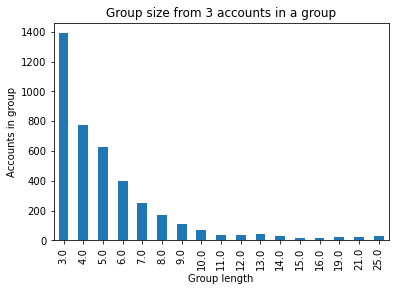
\includegraphics[width=0.2\textwidth]{group_size}\label{fig:f1}}
  \hfill
  \subfloat[Negative]{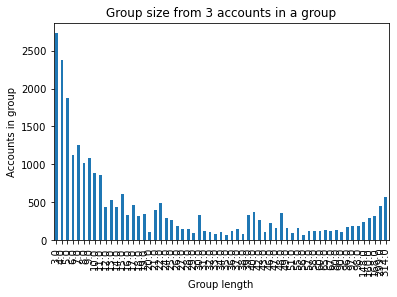
\includegraphics[width=0.2\textwidth]{group_size_negative}\label{fig:f2}}
  \caption{Groups}
\end{figure}


\begin{figure}[H]
  \centering
  \subfloat[Positive]{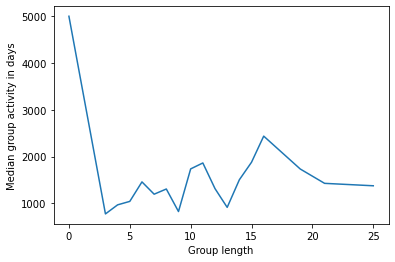
\includegraphics[width=0.2\textwidth]{group_activity}\label{fig:f1}}
  \hfill
  \subfloat[Negative]{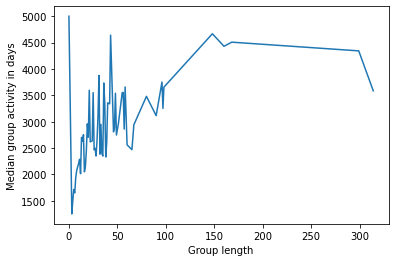
\includegraphics[width=0.2\textwidth]{group_activity_negative}\label{fig:f2}}
  \caption{Activity}
\end{figure}

\begin{figure}[H]
  \centering
  \subfloat[Positive]{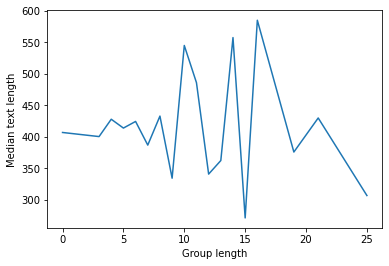
\includegraphics[width=0.2\textwidth]{len_review}\label{fig:f1}}
  \hfill
  \subfloat[Negative]{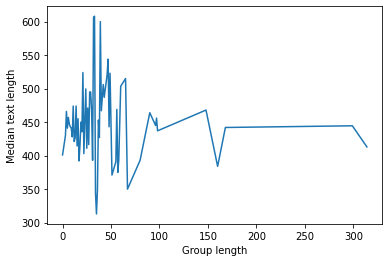
\includegraphics[width=0.2\textwidth]{len_review_negative}\label{fig:f2}}
  \caption{Length}
\end{figure}

\begin{figure}[H]
  \centering
  \subfloat[Positive]{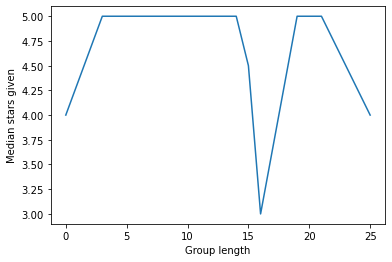
\includegraphics[width=0.2\textwidth]{stars_given}\label{fig:f1}}
  \hfill
  \subfloat[Negative]{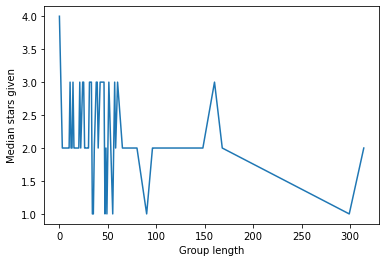
\includegraphics[width=0.2\textwidth]{stars_given_negative}\label{fig:f2}}
  \caption{Stars}
\end{figure}



% insert your bibliographic references into the bib.bib file
\bibliographystyle{plain}
\addcontentsline{toc}{section}{Bibliography}% Add to the TOC
\bibliography{bib}
\end{document}
